\documentclass[11pt, aspectratio=169, xcolor=table,hyphens]{beamer}
\usepackage[utf8]{inputenc}
\usepackage[T1]{fontenc}
\usepackage{lmodern}
\usepackage[spanish]{babel}
\usetheme{Berlin}
\usepackage{pdfrender}
\usepackage{tikz}
\usepackage{graphicx}
\usepackage{xcolor}
\usepackage{hyperref}
\usepackage{cite} %permite salto de línea en referencias largas
\usepackage{ragged2e}
\renewcommand{\raggedright}{\justifying}
\usepackage{smartdiagram}
\usepackage[version=4]{mhchem}
\usepackage{chemfig}

\begin{document}
\author{Prof. Daniel Muñoz \\
	\texttt{daniel.munoz3@mail.udp.cl}}
\title{Química}
\subtitle{Clase 2}
\institute{Universidad Diego Portales}
\titlegraphic{\includegraphics[width=4cm]{../img/udplogo}}
\date{\today} %para mostrar el día de la compilación borrar esta línea.

%	\begin{frame}[plain]
\maketitle
%	\end{frame}

\begin{frame}{Tópicos}
	\tableofcontents
\end{frame}

\section{Tabla periódica y electronegatividad.}
\label{sec:org508fefb}
\begin{frame}[label={sec:orgdb10a88}]{¿Qué es la TP? un poco de historia: J. Döbereiner \cite{Lifeder2022}}
	\begin{columns}
		\begin{column}{0.5\columnwidth}
			\begin{itemize}
				\item <1-> J.W. Döbereiner, científico alemán fue el primero que propuso un ordenamiento, las llamadas \emph{triadas} de elementos.
				\item <2-> Descubrió que si se promedian los \emph{pesos equivalentes} de ciertos elementos (por ejemplo óxidos de\ldots{}) se obtiene, aproximadamente la masa de un tercer elemento.
			\end{itemize}
		\end{column}
		\begin{column}{0.5\columnwidth}
			\only<1>{
				\begin{figure}[htbp]
					\centering
					\includegraphics[width=0.5\textwidth]{../img/dobereiner.jpeg}
					\caption{J.W. Döbereiner 1780-1849}
				\end{figure}
			}

			\only<2>{
				\begin{itemize}
					\item \(SrO = \frac{CaO + BaO}{2} = \frac{59+155}{2} = 107\)
					\item \(Br = \frac{Cl + I}{2} = \frac{35.5+127}{2} = 81,25\)
					\item \(Na = \frac{Li + K}{2} = \frac{7+39}{2} = 23.0\)
				\end{itemize}
			}
		\end{column}
	\end{columns}
\end{frame}
\begin{frame}[label={sec:org248f57a}]{Un poco de historia. Newlands \cite{Nuclear2023}}
	\begin{columns}
		\begin{column}{0.5\columnwidth}
			\begin{itemize}[<+->]
				\item J Newlands, químico inglés que desarrollo el primer esbozo de la ley periódica, la ley de las octavas.
				\item Se percató que cuando se ordenan los elementos según su peso equivalente hay un incremento aproximado de 7 unidades, y una repetición de sus propiedades químicas cada 8 elementos
			\end{itemize}
		\end{column}
		\begin{column}{0.5\columnwidth}
			\only<1>{
				\begin{figure}[htbp]
					\centering
					\includegraphics[width=0.5\textwidth]{../img/newlands.jpg}
					\caption{J. Newlands, químico inglés 1837 - 1898}
				\end{figure}
			}

			\only<2>{
				\begin{figure}[htbp]
					\centering
					\includegraphics[width=\textwidth]{../img/octavas.jpg}
					\caption{1864 Publica \guillemotleft{}On the Law of Octaves\guillemotright{}}
				\end{figure}
			}
		\end{column}
	\end{columns}
\end{frame}
\begin{frame}[label={sec:orga6ab8bb}]{Mendeléyev, El padre de la Tabla periódica \cite{Scerri2007}.}
	\begin{columns}
		\begin{column}{0.5\columnwidth}
			\footnotesize
			\begin{itemize}[<+->]
				\item El padre de la TP y el gran hito fue marcado por el Profesor ruso Dmitri Mendeléyev.
				\item Intentando desarrollar de un modelo para enseñar los elementos conocidos hasta la fecha, Mendeléyev encontró ciertas regularidades en los elementos cuando se ordenan por sus masas.
				\item Utilizando, esta idea de regularidad (ahora conocida como \emph{ley periódica}), se aventuró a predecir el descubrimiento de varios elementos, entre ellos: Eka-aluminio, Eka-silicio.
			\end{itemize}
		\end{column}
		\begin{column}{0.5\columnwidth}
			\only<1>{
				\begin{figure}[htbp]
					\centering
					\includegraphics[width=0.5\textwidth]{../img/mendeleev.jpg}
					\caption{D. Mendeléyev (1834 - 1907)}
				\end{figure}
			}

			\only<2>{
				\begin{figure}[htbp]
					\centering
					\includegraphics[width=0.5\textwidth]{../img/1TP.png}
					\caption{La TP propuesta por Mendeléyev, se pueden apreciar diferentes espacios en vacíos.}
				\end{figure}
			}

			\only<3>{
				\begin{center}
					\begin{tabular}{lll}
						Propiedad           & Eka-aluminio & Galio       \\
						\hline
						Masa                & 68           & 69.723      \\
						Densidad (g/cm³)    & 6.0          & 5.91        \\
						T. Fusión (°C)      & Baja         & 29.76       \\
						Formula del Oxido   & \ce{Ea2O3}   & \ce{Ga2O3}  \\
						Formula del cloruro & \ce{Ea2Cl6}  & \ce{Ga2Cl6} \\
						Presión de vapor    & Volátil      & Volátil     \\
					\end{tabular}
				\end{center}
			}
		\end{column}
	\end{columns}
\end{frame}
\begin{frame}[label={sec:org4188d59}]{En la actualidad.}
	\begin{columns}
		\begin{column}{0.5\columnwidth}
			\begin{itemize}[<+->]
				\item Existen muchos Sistemas Periódicos (no todos son tablas).
				\item Cada uno de ellos tiene un uso diferente.
			\end{itemize}
		\end{column}
		\begin{column}{0.5\columnwidth}
			\only<2>{
				\begin{figure}[htbp]
					\centering
					\includegraphics[width=0.5\textwidth]{../img/benfley.png}
					\caption{Espiral de Benfley 1964.}
				\end{figure}
			}

			\only<3>{
				\begin{figure}[htbp]
					\centering
					\includegraphics[width=0.5\textwidth]{../img/morgan.png}
					\caption{Hidrógeno central de Jeff Morgan.}
				\end{figure}
			}

			\only<4>{
				\begin{figure}[htbp]
					\centering
					\includegraphics[width=0.5\textwidth]{../img/stowe.png}
					\caption{Capas 3D de Timothy Stowe.}
				\end{figure}
			}

			\only<5>{
				\begin{figure}[htbp]
					\centering
					\includegraphics[width=0.3\textwidth]{../img/tsimmerman.png}
					\caption{Columnas de Valery Tsimmerman 2006.}
				\end{figure}
			}
		\end{column}
	\end{columns}
\end{frame}
\begin{frame}[label={sec:org39b1c4b}]{La \guillemotleft{}clásica\guillemotright{}: 18 grupos (columnas) y 7 períodos (filas):}
	\begin{center}
		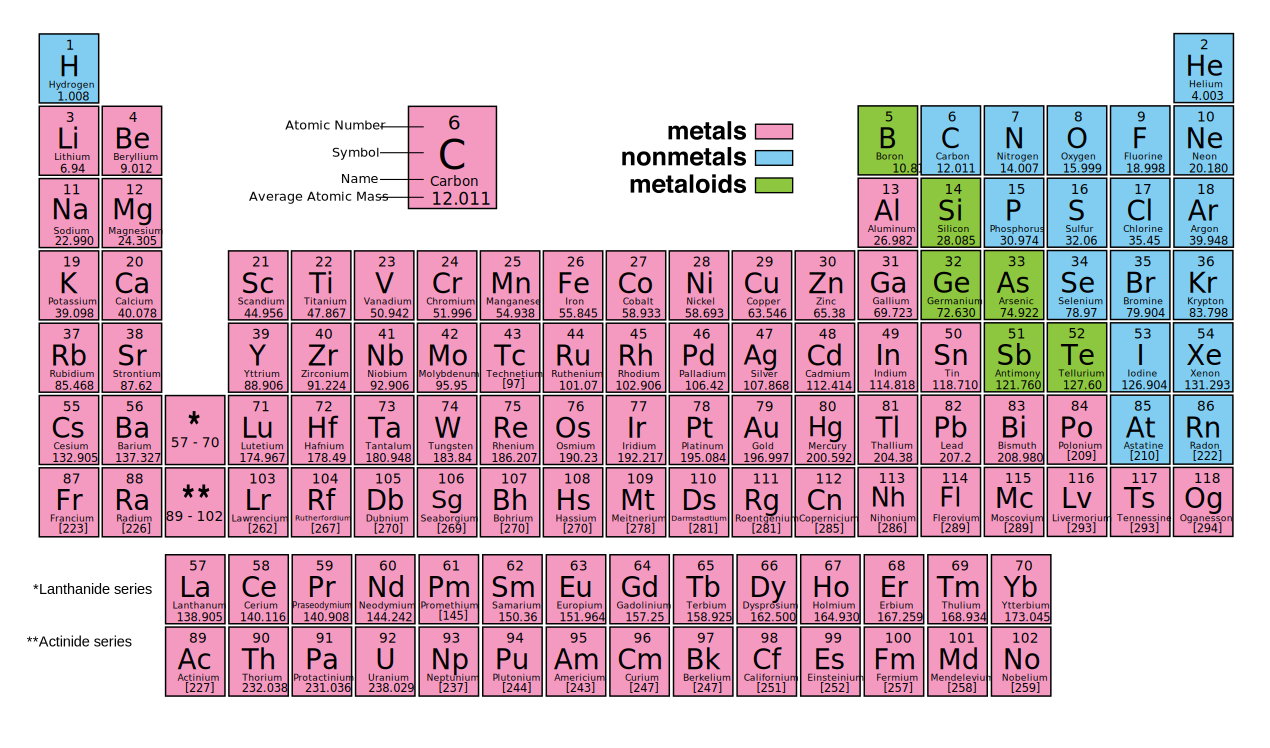
\includegraphics[width=0.7\textwidth]{../img/pte.png}
	\end{center}
\end{frame}
\begin{frame}[label={sec:org320e33d}]{Algunos apuntes de la TP que debe conocer:}
	\begin{center}
		\begin{tabular}{lll}
			                       & Nombre               & Bloque \\
			\hline
			IA                     & Metales Alcalinos    & s      \\
			IIA                    & M. Alcalinos Térreos & s      \\
			IIIA                   & Boroídeos            & p      \\
			IVA                    & Carbonoides          & p      \\
			VA                     & Calcógenos           & p      \\
			VIA                    & Anfígenos            & p      \\
			VIIA                   & Halógenos            & p      \\
			0                      & Gases nobles         & p      \\
			Grupos B               & Transición           & d      \\
			Grupos A               & Representativos      & sp     \\
			Lantánidos y actínidos & Transición interna   & f      \\
		\end{tabular}
	\end{center}
\end{frame}
\begin{frame}[label={sec:org812db5d}]{¿Qué propiedades de los elementos varían a lo largo y ancho de la Tabla periódica?}
	\begin{columns}
		\begin{column}{0.5\columnwidth}
			\footnotesize
			\begin{itemize}[<+->]
				\item Existen muchas propiedades que varían a lo largo y ancho de la TP, a esas propiedades se les conoce como \emph{Propiedades periódicas}.
				\item En este curso solamente estudiaremos la \emph{Electronegatividad}.
				\item Electronegatividad: Tendencia de un elemento para atraer electrones [en un enlace].
				\item Existen, principalmente, dos escalas de electronegatividad, de Mulliken y Pauli. Usaremos la escala de Pauli la cual toma valores desde: 0,7 a 4 (sin unidades)
			\end{itemize}
		\end{column}
		\begin{column}{0.5\columnwidth}
			\begin{figure}[htbp]
				\centering
				\includegraphics[width=\textwidth]{../img/en.jpeg}
				\caption{Variación en aumento de la EN a lo largo y ancho de la TP}
			\end{figure}
		\end{column}
	\end{columns}
\end{frame}
\begin{frame}[label={sec:orgb2afbfb}]{Configuración electrónica y TP}
	\begin{itemize}
		\item Habrá notado que si el elemento posee muchos electrones la configuración electrónica puede tornarse muy larga de escribir, ejemplo:
		\item \ce{_38Sr} = $1s^2 2s^2 2p^6 3s^2 3p^6 4s^2 3d^{10} 4p^6 5s^2$
		\item En química, los electrones que participan en las reacciones químicas son los del \emph{último nivel}, dichos electrones reciben el nombre de \alert{electrones de valencia} (ev), mientras que los \guillemotleft{}otros\guillemotright{} corresponden al \guillemotleft{}kernel\guillemotright{}.
		\item Es por ello que para escribir CE que resalten solo a los ev utilizamos el gas noble anterior más próximo para resumir el \guillemotleft{}kernel\guillemotright{} con ello la configuración anterior quedará:
		\item \ce{_38Sr} = [Kr]5s²
	\end{itemize}
\end{frame}

\section{Enlace Químico}

\begin{frame}{¿Qué es un enlace?}

	\begin{columns}
		\begin{column}{.5\textwidth}
			\begin{itemize}[<+->]
				\item Un enlace se define como la unión de dos átomos (o grupo) que conlleva a la formación de una entidad molecular independiente y estable. \cite{IUPAC2025}
				\item Revisaremos 3 tipos de enlace
				      \begin{itemize}[<+->]
					      \item Metálico
					      \item Iónico
					      \item Covalente
				      \end{itemize}
			\end{itemize}
		\end{column}

		\begin{column}{.5\textwidth}
			\begin{figure}[ht]
				\centering
				\includegraphics<1-2>[width=\textwidth]{../img/bond.jpeg}
				\only<1-2>{\caption{Imágen del benceno utilizando Microscopía de fuerza atómica}}
				\includegraphics<3>[width=\textwidth]{../img/metal.jpg}
				\only<3>{\caption{Vigas metálicas}}
				\includegraphics<4>[width=\textwidth]{../img/sal.jpeg}
				\only<4>{\caption{Sal (cristal de halita)}}
				\includegraphics<5>[width=\textwidth]{../img/coal.jpeg}
				\only<5>{\caption{Carbón}}
			\end{figure}
		\end{column}
	\end{columns}
\end{frame}

\begin{frame}{Enlace metálico}
	\begin{columns}
		\begin{column}{.5\textwidth}
			\begin{itemize}[<+->]
				\item El enlace metálico se da porque los electrones ceden sus electrones de valencia a todos los elementos del conjunto.
				\item Esta deslocalización de los electrones de debe a: la baja electronegatividad
			\end{itemize}
		\end{column}

		\begin{column}{.5\textwidth}
			\begin{figure}[ht]
				\centering
				\includegraphics[width=\textwidth]{../img/sea-electron.png}
				\caption{Teoría del \textit{Mar de electrones}}
			\end{figure}

		\end{column}
	\end{columns}

\end{frame}

\begin{frame}{Enlace Iónico}
	\begin{columns}
		\begin{column}{.5\textwidth}
			\begin{itemize}[<+->]
				\item El enlace iónico se da entre un elemento metálico y otro no-metálico.
				\item Una determinación más cuantitativas es si $\Delta EN > 1,7 $
				\item Una característica que aquí existe una cesión de electrones del metal al no-metal.
				\item De esta forma dejando al metal como \textit{catión} y al no-metal como \textit{anión}.
				\item La transferencia de electrones se da en la medida que ambos elementos queden con una \textbf{capa llena}.
			\end{itemize}
		\end{column}

		\begin{column}{.5\textwidth}
			\begin{figure}[ht]
				\centering
				\includegraphics[width=\textwidth]{../img/ionico.jpg}
				\caption{Explicación de la formación del LiF}
			\end{figure}

		\end{column}
	\end{columns}
\end{frame}

\begin{frame}{Enlace Covalente}
	\begin{columns}
		\begin{column}{.5\textwidth}
			\begin{itemize}[<+->]
				\item El enlace covalante se entre la unión de dos no-metales.
				\item En este tipo de enlaces se dice que ocurren cuando $\Delta EN < 1,7 $
				\item Dado que la diferencia de EN es pequeña, ambos elementos compiten por los electrones del otro.
				\item Existen dos tipos de enlace covalente:
				      \begin{itemize}[<+->]
					      \item Si $\Delta EN = 0$, entonces sera un enlace covalente \textbf{apolar}.
					      \item En caso contrario será un enlace covalente \textbf{polar}.
				      \end{itemize}
			\end{itemize}
		\end{column}

		\begin{column}{.5\textwidth}
			\begin{figure}[ht]
				\centering
				\includegraphics[width=\textwidth]{../img/cl2.png}
			\end{figure}

		\end{column}
	\end{columns}

\end{frame}

\begin{frame}{Estructuras de Lewis}
	\begin{columns}
		\begin{column}{.5\textwidth}
			\begin{itemize}[<+->]
				\item El nombre de Estructuras de Lewis deben el nombre a Gilber N. Lewis
				\item Científico de EEUU que en 1916 formula la \textit{regla del octeto}.
				\item Lewis desarrollo toda su teoría aún sin conocer todo el desarrollo mecanocuántico que explica en el enlace químico y, aún así usamos sus ideas hasta el día de hoy.
			\end{itemize}
		\end{column}

		\begin{column}{.5\textwidth}
			\begin{figure}[ht]
				\centering
				\includegraphics[height=0.6\textheight]{../img/lewis}
				\caption{Gilber N. Lewis 1875 - 1946}
			\end{figure}

		\end{column}
	\end{columns}

\end{frame}

\begin{frame}{Simbolos de Lewis}
	\begin{columns}
		\begin{column}{.5\textwidth}
			\begin{itemize}[<+->]
				\item Primero que todo: \textbf{solo trabajaremos con elementos representativos}
				\item Para construir una estructura de Lewis, primero se dibujarán los \textit{símbolos de lewis}.
				\item Para dibujar un símbolo de lewis bastará con rodear al elemento en sus cuatro costados con tantos puntos como electrones de valencia tenga: ejemplo Cl, Grupo VIIA = 7 e^- de valencia.
			\end{itemize}
		\end{column}

		\begin{column}{.5\textwidth}
		  \Huge
			\centering
			\only<3>{
				\Charge{0=\.}{Cl}
			}
			\only<4>{
				\Charge{0=\., 90=\.}{Cl}
			}
			\only<5>{
				\Charge{0=\., 90=\., 180=\.}{Cl}
			}
			\only<6>{
				\Charge{0=\., 90=\., 180=\., 270=\.}{Cl}
			}
			\only<7>{
				\Charge{0=\:, 90=\., 180=\., 270=\.}{Cl}
			}
			\only<8>{
				\Charge{0=\:, 90=\:, 180=\., 270=\.}{Cl}
			}
			\only<9>{
				\Charge{0=\:, 90=\:, 180=\:, 270=\.}{Cl}
			}
		\end{column}
	\end{columns}

\end{frame}

\begin{frame}{Estructuras de Lewis}
  \begin{columns}
	\begin{column}{.5\textwidth}
	  \begin{enumerate}[<+->]
	  	\item Contar los ev de todos los átomos en la molécula.
		\item Elegir el átomo central, menos electronegativo (excepto H)
		\item Dibujar enlaces del átomo central a los \textit{ligandos}.
		\item Distribuír los electrones sobrantes al átomo central y después a los \textit{ligandos}.
		  \item Todos los átomos cumplen la \textit{regla del octeto} o \textit{dueto} para el hidrógeno y se conserva el número de electrones del paso 1.
	  \end{enumerate}
	\end{column}

	\begin{column}{.5\textwidth}
	  \centering
	  \only<1>{\ce{CCl_4} = $7 \times 4 + 4 = 32$}
	  \only<2>{C = 2,55 > Cl = 3.16}
	  \only<3>{\chemfig{Cl-[7]C(-[1]Cl)(-[5]Cl)-[7]Cl}}
	  \only<4->{\chemfig{{\Charge{45=\:,135=\:,225=\:}{Cl}}-[7]C(-[1]{\Charge{45=\:,135=\:,315=\:}{Cl}})(-[5]{\Charge{135=\:,225=\:,315=\:}{Cl}})-[7]{\Charge{45=\:,315=\:,225=\:}{Cl}}}}
	\end{column}
  \end{columns}

\end{frame}

\begin{frame}{Otros tipos de enlaces}
  \begin{columns}
	\begin{column}{.5\textwidth}
	  \begin{itemize}[<+->]
\item A veces para que el átomo central o los ligandos puedan cumplir el \textit{octeto} será necesario tener más de un par de electrones en el enlace, a veces, puede ser:
  \begin{itemize}[<+->]
\item Dos pares, y se llamará \textit{enlace doble}
  \item Tres pares, u se llamará \textit{enlace triple}
  \end{itemize}
	  \end{itemize}
	\end{column}

	\begin{column}{.5\textwidth}
	  \begin{figure}[ht]
		\centering
		\only<2>{
		\chemfig{\Charge{135=\:,225=\:}{O}=C=\Charge{45=\:,315=\:}{O}}
		\caption{\ce{CO_2}}
		}
		\only<3>{
		  \chemfig{H-C~\Charge{0=\:}{N}}
		  \caption{\ce{HCN}}
		}
	  \end{figure}

	\end{column}
  \end{columns}

\end{frame}

\begin{frame}[allowframebreaks]{Bibliografía}
	\begin{thebibliography}{Scerri, 2007}
		\footnotesize
		\setbeamertemplate{bibliography item}[online]
		\bibitem[Labnews, 2019]{Labnews2019}
		Laboratory news
		\newblock \emph{Alternative periodic tables}
 		\newblock \url{https://www.labnews.co.uk/article/2029799/alternative-periodic-tables}

		\setbeamertemplate{bibliography item}[online]
		\bibitem[Lifeder, 2022]{Lifeder2022}
		Lifeder
		\newblock \emph{Tríadas de Döbereiner}
		\newblock \url{https://www.lifeder.com/triadas-de-dobereiner/}

		\setbeamertemplate{biblography item}[online]
		\bibitem[Energía Nuclear, 2023]{Nuclear2023}
		Energía Nuclear
		\newblock \emph{Ley de las Octavas de Newlands}
		\newblock \url{https://energia-nuclear.net/quimica/tabla-periodica/linea-del-tiempo/ley-de-las-octavas}

		\setbeamertemplate{bibliography item}[book]
		\bibitem[Scerri, 2007]{Scerri2007}
		Scerri, Eric.
		\newblock \emph{The Periodic Table: It's Story and Its Significance}
		\newblock Oxford University Press, 2007

		\setbeamertemplate{bibliography item}[online]
		\bibitem[IUPAC, 2025]{IUPAC2025}
		International Union of Pure and Applied Chemistry
		\newblock \emph{IUPAC Compendium of Chemical Terminology, 5th ed.}
		\newblock \url{https://doi.org/10.1351/goldbook.CT07009}


	\end{thebibliography}
\end{frame}
\
\end{document}
